\documentclass{article}

\usepackage{xcolor}

\usepackage{tikz}
\usetikzlibrary{automata, positioning, arrows}

\usepackage{circuitikz}

\usepackage{geometry}
\geometry {
    top=20mm,
    bmargin=25mm,
}

\usepackage{subfig}
\usepackage{subcaption}


\begin{document}

\title{ciao}
\author{riciao,  ririciao}
\maketitle

\begin{figure}[ht] % ’ht’ tells LaTeX to place the figure ’here’ or at the top of the page
    \centering % centers the figure

    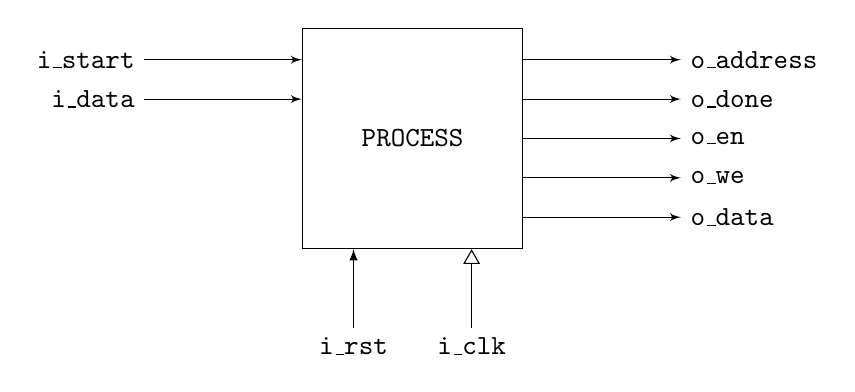
\begin{tikzpicture}[node distance = 5mm and 15mm]
        \node (comp) [draw,minimum size=28mm] {\texttt{PROCESS}};
        % in
        \coordinate[above left= 10mm and 20mm of comp.west]  (i1);
        \foreach \i [count=\xi from 1] in {2} 
            \coordinate[below=of i\xi]  (i\i);
        \foreach \i [count=\xi from 1] in {\texttt{i\_start}, \texttt{i\_data}}
            \draw[-latex']  (i\xi) node[left] {\i} -- (i\xi-| comp.west);
        %under
        \coordinate[below right = 10mm and 7.5mm of comp.south]  (u1);
        \foreach \i [count=\xi from 1] in {2} 
            \coordinate[left=of u\xi]  (u\i);
        %\foreach \i [count=\xi from 1] in {\texttt{i\_clk}, \texttt{i\_rst}}
            \draw[-open triangle 60]  (u1) node[below] {\texttt{i\_clk}} -- (u1 |- comp.south);
            \draw[-latex]  (u2) node[below] {\texttt{i\_rst}} -- (u2 |- comp.south);
            
        % out
        \coordinate[above right= 10mm and 20mm of comp.east]  (o1);
        \foreach \i [count=\xi from 1] in {2,...,5} 
            \coordinate[below=of o\xi]  (o\i);
        \foreach \i [count=\xi from 1] in {\texttt{o\_address}, \texttt{o\_done},
                                                    \texttt{o\_en}, \texttt{o\_we}, \texttt{o\_data}}
            \draw[-latex'] (comp.east |- o\xi) -- (o\xi) node[right] {\i};
        %
        \end{tikzpicture}

    \caption{schema del componente realizzato}
    \label{fig:component}
\end{figure}


\tikzset{ flipflop myJK/.style={
    flipflop,
    flipflop def={t1=\texttt{i\_start}, t2=\texttt{i\_data}, t3=\texttt{i\_clk}, t6=Q, t4={\ctikztextnot{Q}}, c3=1}}
}




\begin{figure}
    \centering
    \begin{circuitikz}
        \ctikzset{multipoles/thickness=3.5}
        \ctikzset{multipoles/dipchip/width=4}
        %sinistra
        \draw   (0,0) node[dipchip,
                num pins=10, hide numbers, no topmark,
                external pins width=0](C){\large{\texttt{COMPONENT}}};
        \node   [right] at (C.bpin 1) {\texttt{i\_start}};
        \draw   (C.bpin 1) -- ++(-1,0) coordinate(extpin);
        \node   [right] at (C.bpin 2) {\texttt{i\_data}};
        \draw   (C.bpin 2) -- ++(-1,0) coordinate(extpin);
        \node   [right] at (C.bpin 4) {\texttt{i\_rst}};
        \draw   (C.bpin 4) -- ++(-1,0) coordinate(extpin);
        \draw   (C.bpin 5) ++(0,0.2) -- ++(0.2,-0.2)
                node[right]{\texttt{i\_clk}} -- ++(-0.2,-0.2);
        \draw   (C.bpin 5) -- ++(-1,0) coordinate(extpin);
        %destra
        \node   [left] at (C.bpin 6) {\texttt{o\_data}};
        \draw   (C.bpin 6) -- ++(1,0) coordinate(extpin);
        \node   [left] at (C.bpin 7) {\texttt{o\_done}};
        \draw   (C.bpin 7) -- ++(1,0) coordinate(extpin);
        \node   [left] at (C.bpin 8) {\texttt{o\_en}};
        \draw   (C.bpin 8) -- ++(1,0) coordinate(extpin);
        \node   [left] at (C.bpin 9) {\texttt{o\_we}};
        \draw   (C.bpin 9) -- ++(1,0) coordinate(extpin);
        \node   [left] at (C.bpin 10) {\texttt{o\_address}};
        \draw   (C.bpin 10) -- ++(1,0) coordinate(extpin);
        \end{circuitikz}
\end{figure}
\pagebreak

\begin{figure}[ht]
    \centering 
    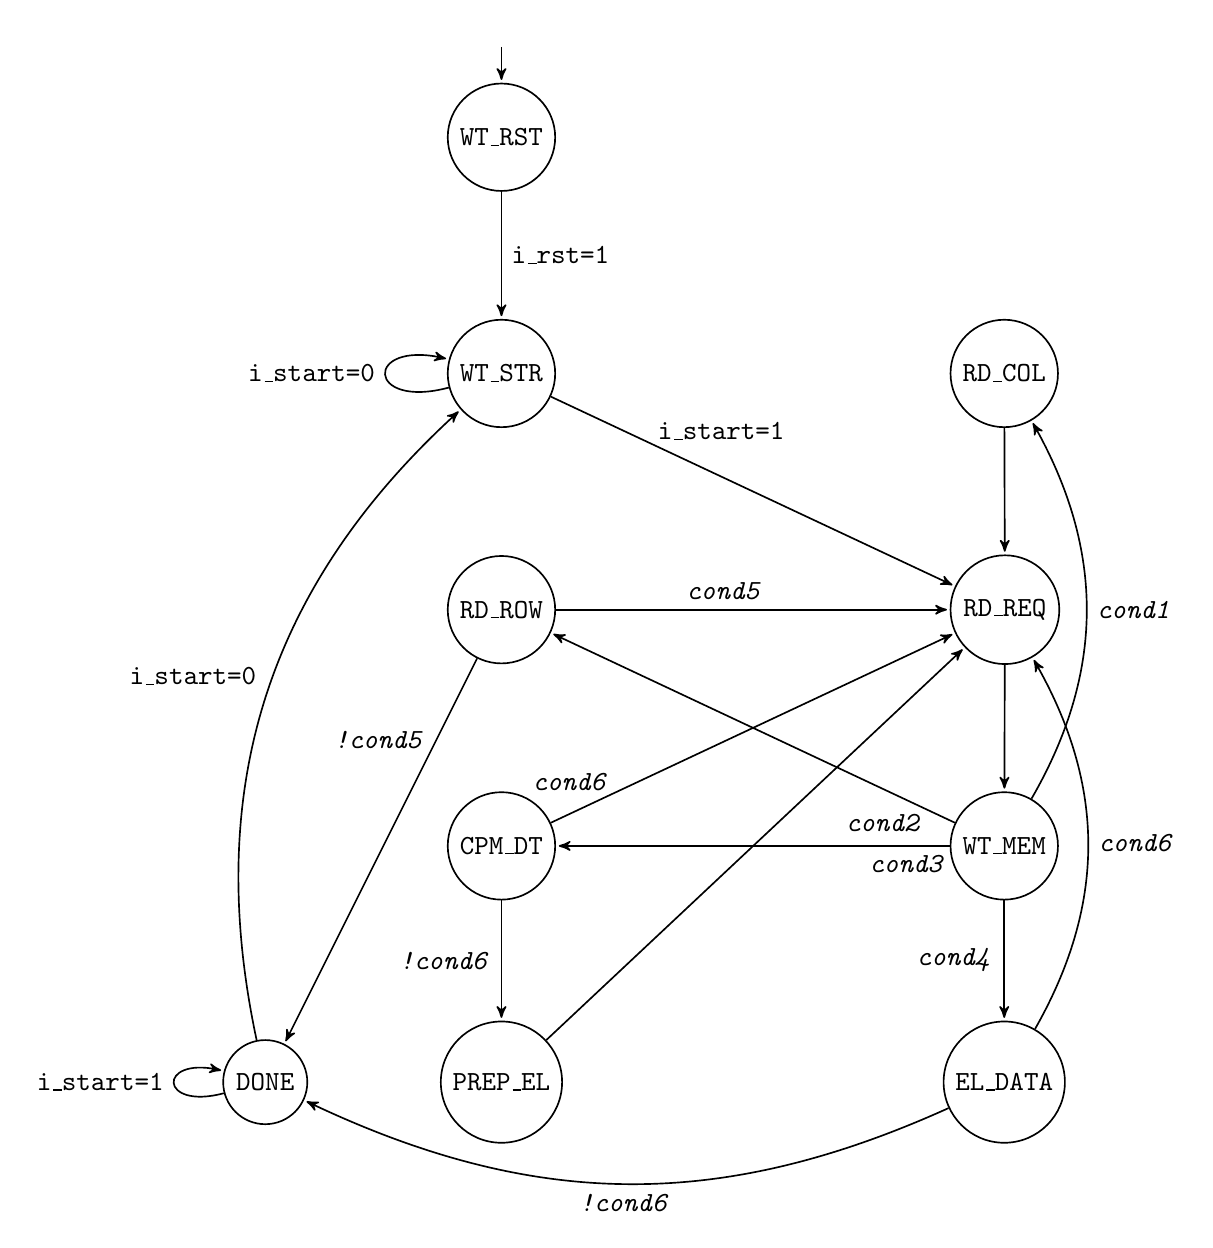
\begin{tikzpicture}[->,>=stealth',shorten >=1pt,auto,node distance=3cm,
        semithick, initial text=$ $, initial where= above]

        \node[state, initial]           (0) {\texttt{WT\_RST}};
        \node[state, below of=0]        (1) {\texttt{WT\_STR}};
        \node[state, right=5cm of 1]    (2) {\texttt{RD\_COL}};
        \node[state, below of=1]        (3) {\texttt{RD\_ROW}};
        \node[state, below of=3]        (4) {\texttt{CPM\_DT}};
        \node[state, right=5cm of 3]    (5) {\texttt{RD\_REQ}};
        \node[state, right=5cm of 4]    (6) {\texttt{WT\_MEM}};
        \node[state, below of=4]        (7) {\texttt{PREP\_EL}};
        \node[state, below of=6]        (8) {\texttt{EL\_DATA}};
        \node[state, left of=7]         (9) {\texttt{DONE}};

        \draw   (0) edge                    node {\texttt{i\_rst=1}}                                            (1)
                (1) edge[loop left]         node {\texttt{i\_start=0}}                                          (1)
                (1) edge                    node [yshift=15pt, xshift=-38pt]{\texttt{i\_start=1}}               (5)
                (2) edge                    node {}                                                             (5)
                (3) edge                    node [xshift=-10pt] {\texttt{\emph{cond5}}}                         (5)
                (3) edge[left]              node [yshift=40pt, xshift=20pt]{\texttt{\emph{!cond5}}}             (9)
                (4) edge                    node [at start, yshift=8pt, xshift=25pt] {\texttt{\emph{cond6}}}    (5)
                (4) edge                    node[left] {\texttt{\emph{!cond6}}}                                 (7)
                (5) edge                    node {}                                                             (6)
                (6) edge[bend right, right] node {\texttt{\emph{cond1}}}                                        (2)
                (6) edge[right]             node [at start, xshift=-43pt] {\texttt{\emph{cond2}}}               (3)
                (6) edge                    node [at start, xshift=-15pt] {\texttt{\emph{cond3}}}               (4)
                (6) edge[left]              node {\texttt{\emph{cond4}}}                                        (8)                
                (7) edge                    node {}                                                             (5)
                (8) edge[bend right]        node[right]  {{\texttt{\emph{cond6}}}}                              (5)
                (8) edge[bend left=25]      node {{\texttt{\emph{!cond6}}}}                                     (9)  
                (9) edge[bend left]         node {\texttt{i\_start=0}}                                          (1)
                (9) edge[loop left]         node {\texttt{i\_start=1}}                                          (9);

    \end{tikzpicture}
    \caption{Diagramma degli stati della macchina a stati finiti utilizzata}
    \label{fig:fsm}
\end{figure}

Le condizioni utilizzate nel processo sono le seguenti:

\begin{center}
    \begin{tabular}{||c|c||}
        %\hline
        \hline
        \texttt{\emph{cond1}} & \texttt{count $=$ 0} \\
        \hline
        \texttt{\emph{cond2}} & \texttt{count $=$ 1} \\
        \hline
        \texttt{\emph{cond3}} & \texttt{shift\_level $=$ 3 (non ancora calcolato)} \\
        \hline
        \texttt{\emph{cond4}} & \texttt{\emph{!cond1} \&\& \emph{!cond2} \&\& \emph{!cond3}} \\   
        \hline
        \texttt{\emph{cond5}} & \texttt{n\_col $\cdot$ n\_row $>$ 0} \\
        \hline
        \texttt{\emph{cond6}} & \texttt{count $\leq$ n\_col $\cdot$ n\_row $+$ 2} \\      
        \hline
        %\hline
        \end{tabular}
\end{center}

Si ricorda inoltre, che per ogni stato dell'FSM è presente un arco uscente implicito diretto verso lo stato \texttt{WT\_STR}, 
che simboleggia la possibilità di interrompere in qualsiasi momento l'elaborazione dell'immagine corrente, tramite un segnale \texttt{i\_rst $=$ 1}

%con subfig ma non funzionava
\pagebreak
\begin{table}
    \centering
    \caption{Esempio}
    \subfloat[Contenuto della memoria]{
        \begin{tabular}{c|c}
            addr. & data \\
            \hline \hline
            0 & 14      \\
            1 & 12      \\
            2 & 13      \\
            3 & 7       \\
            4 & 13      \\
            5 & 13      \\
            6 & 7       \\
            7 & 13      \\
            8 & 13      \\
            9 & 14      \\
            10 & 12      \\
            12 & 13      \\
            13 & 7       \\
            14 & 13      \\
            15 & 13      \\
            16 & 7       \\
            17 & 13      \\
           \end{tabular}\hspace{0.3cm}
        \begin{tabular}{c|c}
            addr. & data \\
            \hline \hline
            0 & 14      \\
            1 & 12      \\
            2 & 13      \\
            3 & 7       \\
            4 & 13      \\
            5 & 13      \\
            6 & 7       \\
            7 & 13      \\
            8 & 13      \\
            9 & 14      \\
            10 & 12      \\
            12 & 13      \\
            13 & 7       \\
            14 & 13      \\
            15 & 13      \\
            16 & 7       \\
            17 & 13      \\
           \end{tabular}
    }\hspace{0.5cm}
    \subfloat[Immagine sorgente]{
        
\includegraphics[scale=0.2]{immSorg.jpg}
    }\hspace{0.3cm}
    \subfloat[Immagine equalizzata]{
        
\includegraphics[scale=0.2]{immElab.jpg}
    }
  \end{table}

  \pagebreak

  %con subcaption commenta subfig
%   \begin{figure}
%     \begin{minipage}[c]{.35\linewidth}
%     \centering 
%     \begin{tabular}{c|c}
%         addr. & data \\
%         \hline \hline
%         0 & 14      \\
%         1 & 12      \\
%         2 & 13      \\
%         3 & 7       \\
%         4 & 13      \\
%         5 & 13      \\
%         6 & 7       \\
%         7 & 13      \\
%         8 & 13      \\
%         9 & 14      \\
%         10 & 12      \\
%         12 & 13      \\
%         13 & 7       \\
%         14 & 13      \\
%         15 & 13      \\
%         16 & 7       \\
%         17 & 13      \\
%        \end{tabular}
%     \begin{tabular}{c|c}
%         addr. & data \\
%         \hline \hline
%         0 & 14      \\
%         1 & 12      \\
%         2 & 13      \\
%         3 & 7       \\
%         4 & 13      \\
%         5 & 13      \\
%         6 & 7       \\
%         7 & 13      \\
%         8 & 13      \\
%         9 & 14      \\
%         10 & 12      \\
%         12 & 13      \\
%         13 & 7       \\
%         14 & 13      \\
%         15 & 13      \\
%         16 & 7       \\
%         17 & 13      \\
%        \end{tabular}
%     \subcaption{A subfigure}\label{esempio1}
%     \end{minipage}%
%     \begin{minipage}[c]{.3\linewidth}
%     \centering
%         
\includegraphics[scale=0.2]{immSorg.jpg}
%     \subcaption{Another subfigure}\label{esempio2}
%     \end{minipage}
%     \begin{minipage}[c]{.3\linewidth}
%         \centering
%             
\includegraphics[scale=0.2]{immElab.jpg}
%         \subcaption{Another subfigure}\label{esempio3}
%         \end{minipage}
%     \end{figure}

  ciao sono un testo

\end{document}